\documentclass{beamer}
% \linespread{1.3}

\mode<presentation>{
\usetheme{Madrid}
\usecolortheme{default}
%\usecolortheme{beaver}
}
\usepackage[utf8]{inputenc}
\usepackage{utopia}
\usepackage{verbatim}
\usepackage[portuguese]{babel}
\usepackage{pgfplots}
\pgfplotsset{/pgf/number format/use comma,compat=newest}
\usepackage{color}
\usepackage{amsmath,amsfonts,amssymb}
\usepackage{hyperref}
\usepackage{tikz}
\usepackage{caption}
\usepackage{soul}
%https://www.overleaf.com/project/61717826e515873b24296576
\usepackage{graphicx}
\usepackage{algorithm2e}
\usepackage{algorithmic}
\usetikzlibrary{positioning}

\setlength{\parskip}{1em}

\newcommand\ldiaarg[1]{\langle#1\rangle}

\newcommand{\M}{\mathcal{M}}
\newcommand{\LL}{\mathcal{L}} %for automata

\newcommand{\POL}{\mathsf{POL}}
\newcommand{\Decide}{\mathsf{Decide}}
\newcommand{\DecidePSPACE}{\mathsf{mcPOL}}
\newcommand{\reach}{\mathsf{PSPACEReach}}
\newcommand{\CreateDelta}{\mathsf{CreateDelta}}
\newcommand{\StringRepresent}{\mathsf{StringRepresent}}
\newcommand{\StoreStrings}{\mathsf{StoreStrings}}
\newcommand{\ResidueByLetter}{\mathsf{ResidueByLetter}}
\newcommand{\ResidueByWord}{\mathsf{ResidueByWord}}
\newcommand{\AuxOut}{\mathsf{AuxOut}}
\newcommand{\GetSetNP}{\mathsf{GetSetNP}}
\newcommand{\T}{\mathsf{True}}
\newcommand{\Fa}{\mathsf{False}}
\newcommand{\tr}{\mathsf{tr}}
\newcommand{\starfree}{\mathsf{Star\mbox{-}Free}}
\newcommand{\word}{\mathsf{Word}}
\newcommand{\existential}{\mathsf{Existential}}
\newcommand{\PSPACE}{\mathsf{PSPACE}}
\newcommand{\NPSPACE}{\mathsf{NPSPACE}}
\newcommand{\PTime}{\mathsf{P}}
\newcommand{\NP}{\mathsf{NP}}
\newcommand{\PTIME}{\mathsf{PTIME}}
\newcommand{\automaton}{\mathcal A}
\newcommand{\modelM}{\mathcal M}
\newcommand{\languageof}[1]{L({#1})}
\newcommand{\set}[1]{\{#1\}}
\newcommand{\suchthat}{\mid}
\newcommand{\union}{\cup}
\newcommand{\Union}{\bigcup}
\newcommand{\ep}{\ensuremath{\varepsilon}}

\newcommand{\obsright}{\blacktriangleright}
\newcommand{\obsleft}{\blacktriangleleft}
\newcommand{\obsup}{\blacktriangle}
\newcommand{\obsdown}{\blacktriangledown}

\newcommand{\expwater}{(\obsright \union \obsup)^* (\obsdown \union \obsleft \union \ep) (\obsright \union \obsup)^*}
\newcommand{\exppower}{(\obsleft \union \obsdown)^* (\obsup \union \obsright \union \ep) (\obsleft \union \obsdown)^*}
\newcommand{\exppatrol}{(\obsright^+ \obsdown^+ \obsleft^+ \obsup^+)^*}

\newcommand\algoaccept{\textbf{accept}}
\newcommand\algoreject{\textbf{reject}}

\tikzstyle{rectNode} = [rectangle, text centered]
\tikzstyle{fastate} = [circle, text centered, draw = black]
\tikzstyle{dots} = [circle, draw = black, fill = black, inner sep=1pt]

\tikzstyle{world} = [draw]

\makeatletter
\let\HL\hl
\renewcommand\hl{%
  \let\set@color\beamerorig@set@color
  \let\reset@color\beamerorig@reset@color
  \HL}
\makeatother



\title[On Verifying Expectations and Observations of Intelligent Agents]{On Verifying Expectations and Observations of Intelligent Agents}
\author{
Sourav Chakraborty\inst{1}
\and
\textbf{Avijeet Ghosh}\inst{1}\and
Sujata Ghosh\inst{1}\and\\
Fran{\c{c}}ois Schwarzentruber\inst{2}}
\institute{\inst{1} Indian Statistical Institute\and \inst{2} Univ Rennes, IRISA}
\date{}

\begin{document}

\begin{frame}
 \maketitle
\end{frame}

\begin{frame}{A Farming Drone}
    \begin{figure}
        \centering
        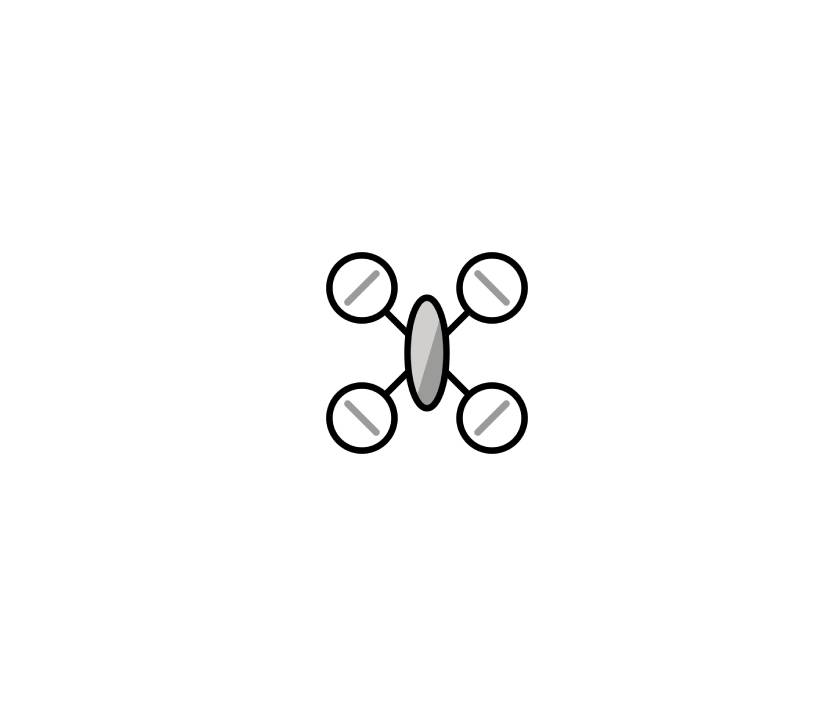
\includegraphics[scale=0.15]{images/drone.jpg}
    \end{figure}
\end{frame}

\begin{frame}{A Farming Drone}
    \begin{figure}
        \centering
        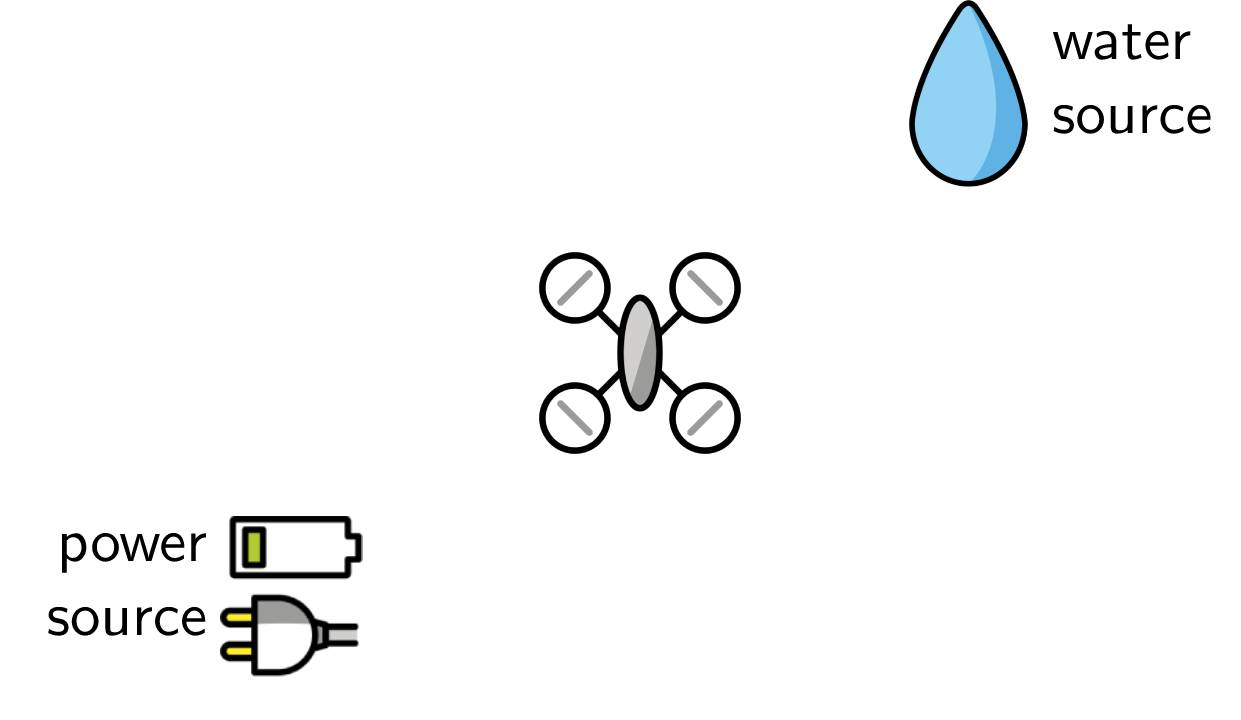
\includegraphics[scale=0.15]{images/drone-water-power.jpg}
    \end{figure}
    \begin{itemize}
        \item A water source on top right corner
        \item A power source on bottom right corner
    \end{itemize}
\end{frame}

\begin{frame}{A Farming Drone}
    \begin{figure}
        \centering
        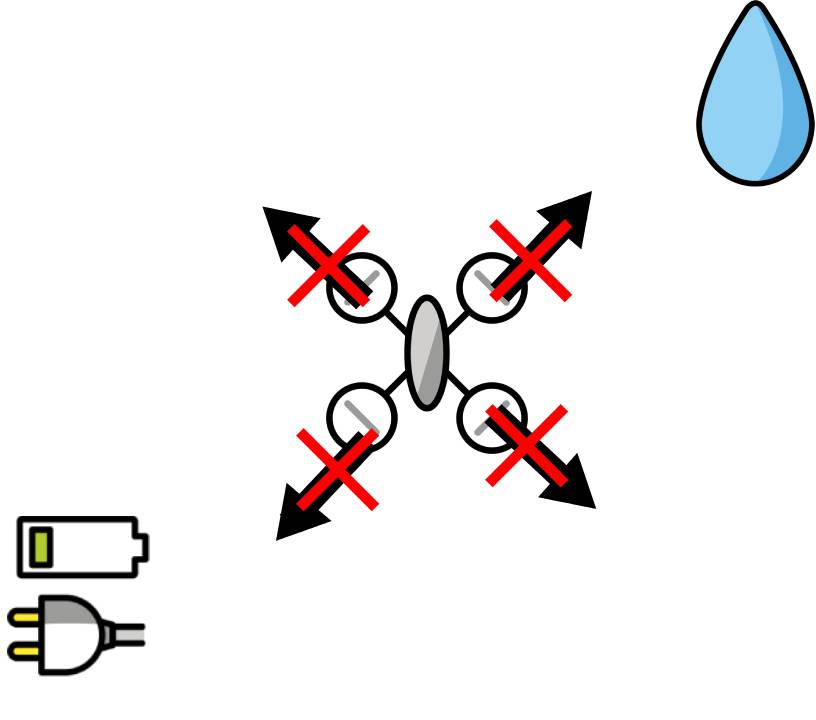
\includegraphics[scale=0.15]{images/no-diag.jpg}
    \end{figure}
    \begin{itemize}
        \item Cannot move diagonally
    \end{itemize}
\end{frame}

\begin{frame}{A Farming Drone}
    \begin{figure}
        \centering
        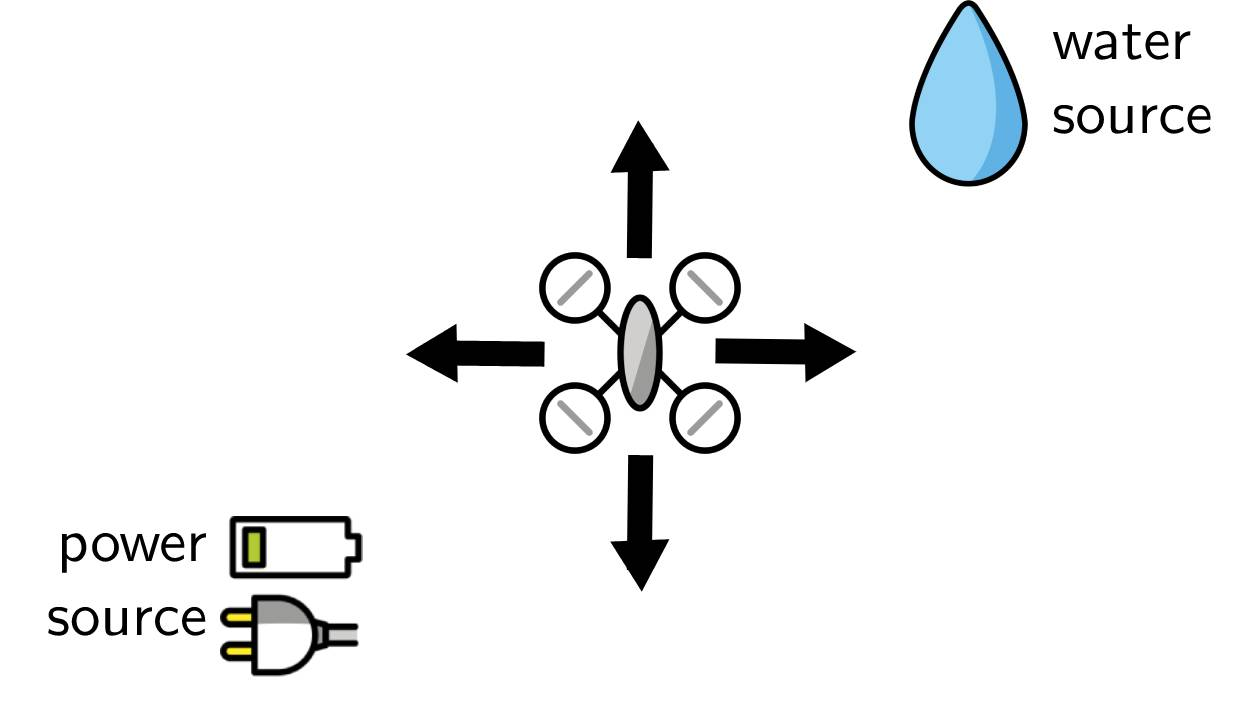
\includegraphics[scale=0.15]{images/drone-move.jpg}
    \end{figure}
    \begin{itemize}
        \item Can move up, down, left or right
    \end{itemize}
\end{frame}

\begin{frame}{Farming Drone: Agents}
    \begin{figure}
        \centering
        
\includegraphics[scale=0.2]{images/a-expects.jpg}
        
\includegraphics[scale=0.2]{images/b-expects.jpg}
    \end{figure}
    \begin{itemize}
        \item Two agents: A and B
    \end{itemize}
\end{frame}

\begin{frame}{Farming Drone: Agents}
    \begin{figure}
        \centering
        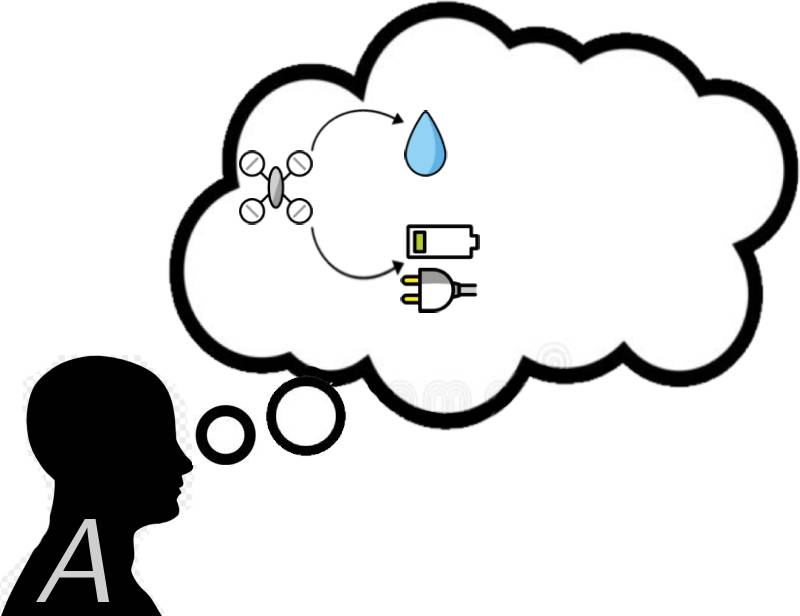
\includegraphics[scale=0.2]{images/a-expects-move.jpg}
        
\includegraphics[scale=0.2]{images/b-expects.jpg}
    \end{figure}
    A expects
    \begin{itemize}
        \item Drone moves towards water or power source with at most one error move.
    \end{itemize}
\end{frame}

\begin{frame}{Farming Drone: Agents}
    \begin{figure}
        \centering
        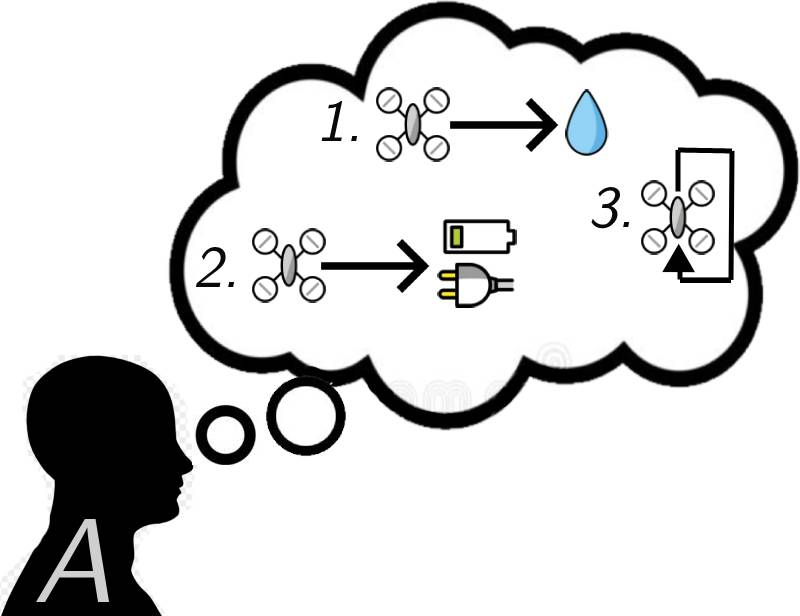
\includegraphics[scale=0.2]{images/a-expects-patrol.jpg}
        
\includegraphics[scale=0.2]{images/b-expects.jpg}
    \end{figure}
    A expects
    \begin{itemize}
        \item Drone moves towards water or power source with at most one error move. 
        \item Drone goes patrolling in clockwise squares.
    \end{itemize}
\end{frame}

\begin{frame}{Farming Drone: Agents}
    \begin{figure}
        \centering
        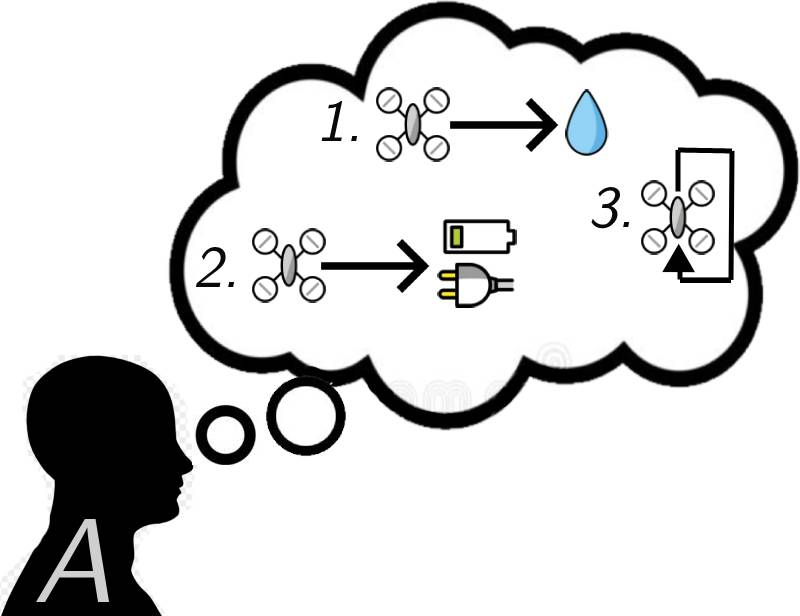
\includegraphics[scale=0.2]{images/a-expects-patrol.jpg}
        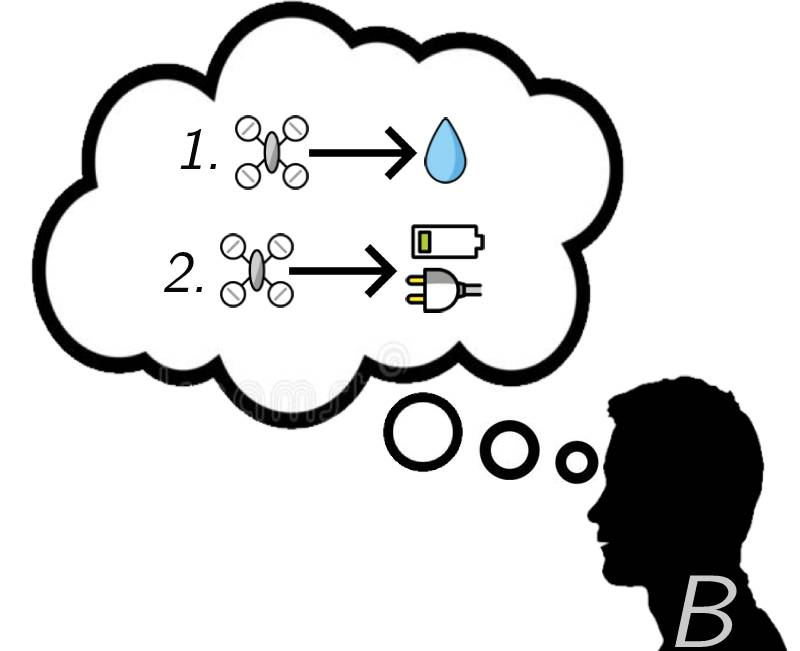
\includegraphics[scale=0.2]{images/b-expects-move.jpg}
    \end{figure}
    B expects
    \begin{itemize}
        \item Drone only moves towards water or power source with at most one error move.
    \end{itemize}
\end{frame}

\begin{frame}{Farming Drone: The Question}
    How to reason in this scenario?\pause
    \begin{itemize}
        \item<2-> After OBSERVING how many steps of drone moves can agent A KNOW drone is moving towards water source?
        \item<3-> How many movements or steps of drone is sufficient to OBSERVE after which no more knowledge will be gained or lost? 
    \end{itemize}
\end{frame}

\begin{frame}{Epistemic Expectation Model}
    \begin{itemize}
        \item Underlying skeleton is Epistemic model $\ldiaarg{S,\sim, V}$.
    \end{itemize}
    \begin{figure}
\begin{tikzpicture}[yscale=1.3]
			\node[world] (s) {$water$};
% 			\node at (-0.1, -0.4) {\tiny $\expwater$};
			\node[world] (t) at (4, 0) {$power$};
% 			\node at (4.3, -0.4) {\tiny $\exppower$};
			\node[world] (u) at (0, 1) {$patrol$};
% 			\node at (2.3, 1) {\tiny $\exppatrol$};
			\node[left = 0mm of s] {$s$};
			\node[right = 0mm of t] {$t$};
			\node[left = 0mm of u] {$u$};
			\draw (s) edge node[above] {$a,b$} (t);
			\draw (s) edge node[left] {$a$} (u);
			\draw (t) edge node[above] {$a$} (u);
		\end{tikzpicture}
\end{figure}
\end{frame}

\begin{frame}{Epistemic Expectation Model}
    \begin{itemize}
        \item Underlying skeleton is Epistemic model $\ldiaarg{S,\sim, V}$.
        \item Along with valuation, each world has a regular expression $\pi$ over a $\Sigma$ assigned representing the \textbf{Expected Observations}. In our model, $\Sigma = \{\obsup, \obsdown, \obsleft, \obsright\}$ representing one step to up, down, left or right respectively.
    \end{itemize}
    \begin{figure}
        \begin{tikzpicture}[yscale=1.3]
			\node[world] (s) {$water$};
			\node at (-0.5, -0.4) {$\small\expwater$};
			\node[world] (t) at (4, 0) {$power$};
			\node at (4.5, -0.4) {$\small\exppower$};
			\node[world] (u) at (0, 1) {$patrol$};
			\node at (2.3, 1) {$\small\exppatrol$};
			\node[left = 0mm of s] {$s$};
			\node[right = 0mm of t] {$t$};
			\node[left = 0mm of u] {$u$};
			\draw (s) edge node[above] {$A,B$} (t);
			\draw (s) edge node[left] {$A$} (u);
			\draw (t) edge node[above] {$B$} (u);
		\end{tikzpicture}
    \end{figure}
\end{frame}

\begin{frame}{Epistemic Expectation Model}
    \begin{itemize}
        \item Underlying skeleton is Epistemic model $\ldiaarg{S,\sim, V}$.
        \item Each world has an assigned regular expression $\pi$ over  $\Sigma$ assigned called the \textbf{Expected Observations}. In our model, $\Sigma = \{\obsup, \obsdown, \obsleft, \obsright\}$ representing one step to up, down, left or right respectively.
        \item Model can get truncated after an observation, say $\obsright\obsdown\obsleft$.
    \end{itemize}
    \begin{figure}
        \begin{tikzpicture}[yscale=1.3]
			\node[world] (s) {$water$};
			\node at (-0.5, -0.4) {\small$\expwater$};
			\node[world] (t) at (4, 0) {$power$};
			\node at (4.5, -0.4) {\small$\exppower$};
			\node[world] (u) at (0, 1) {$patrol$};
			\node at (2.3, 1) {\small$\exppatrol$};
			\node[left = 0mm of s] {$s$};
			\node[right = 0mm of t] {$t$};
			\node[left = 0mm of u] {$u$};
			\draw (s) edge node[above] {$A,B$} (t);
			\draw (s) edge node[left] {$A$} (u);
			\draw (t) edge node[above] {$B$} (u);
		\end{tikzpicture}
    \end{figure}
\end{frame}
 
 \begin{frame}{Epistemic Expectation Model}
    \begin{itemize}
        \item Underlying skeleton is Epistemic model $\ldiaarg{S,\sim, V}$.
        \item Each world has an assigned regular expression $\pi$ over  $\Sigma$ assigned called the \textbf{Expected Observations}. In our model, $\Sigma = \{\obsup, \obsdown, \obsleft, \obsright\}$ representing one step to up, down, left or right respectively.
        \item Model can get truncated after an observation, say $\obsright\obsdown\obsleft$.
    \end{itemize}
    \begin{figure}
         \begin{tikzpicture}[yscale=1.3]
% 			\node[world] (s) {$water$};
% 			\node at (-0.5, -0.4) {$\small\expwater$};
			\node[world] (t) at (4, 0) {$power$};
			\node at (4.5, -0.4) {\small$(\obsleft\union\obsdown)^*$};
			\node[world] (u) at (0, 1) {$patrol$};
			\node at (2.7, 1) {\small$\obsleft^*\obsup^+\exppatrol$};
% 			\node[left = 0mm of s] {$s$};
			\node[right = 0mm of t] {$t$};
			\node[left = 0mm of u] {$u$};
% 			\draw (s) edge node[above] {$A,B$} (t);
% 			\draw (s) edge node[left] {$A$} (u);
			\draw (t) edge node[above] {$B$} (u);
		\end{tikzpicture}
    \end{figure}
\end{frame}
 
\begin{frame}{Public Observation Logic: Syntax}
    The syntax of the Public Observation Logic ($\POL$) has usual boolean and knowledge operator with an extra modality with a regular expression $\pi$:\\
    \vspace{1cm}
    $\begin{array}{r@{\quad::= \quad}l}
		\phi  &
		\top
		\mid
		p
		\mid \neg \phi
		\mid \phi \land \phi
		\mid K_i\phi
		\mid [\pi] \phi,
	\end{array}$\\\pause
	\vspace{1cm}
	The formula $[\pi]\phi$ is interpreted as "After any observation in $\pi$, $\phi$ holds".
\end{frame}

\begin{frame}{Farming Drone}
    \begin{figure}
		\newcommand{\sizefield}{7}
		\begin{tikzpicture}[scale=0.3]
			\foreach \x in {0, 1, ..., \sizefield} {
				\draw (\x, 0) -- (\x, \sizefield);
				\draw (0, \x) -- (\sizefield, \x);
			}
			\node at (0.5, 0.5) {
\includegraphics[width=0.3cm]{images/E097_color.png}};%power
			\node at (6.5, 6.5) {
\includegraphics[width=0.3cm]{images/1F4A7_color.png}};%water
			\node at (3.5, 3.5) {
\includegraphics[width=0.3cm]{images/E1D2_color.png}};%drone
		\end{tikzpicture}
		\begin{tikzpicture}[yscale=1.3]
			\node[world] (s) {$water$};
			\node at (-0.1, -0.4) {\small $\expwater$};
			\node[world] (t) at (4, 0) {$power$};
			\node at (4.3, -0.4) {\small $\exppower$};
			\node[world] (u) at (0, 1) {$patrol$};
			\node at (2.3, 1) {\small $\exppatrol$};
			\node[left = 0mm of s] {$s$};
			\node[right = 0mm of t] {$t$};
			\node[left = 0mm of u] {$u$};
			\draw (s) edge node[above] {$a,b$} (t);
			\draw (s) edge node[left] {$a$} (u);
			\draw (t) edge node[above] {$a$} (u);
		\end{tikzpicture}
    \end{figure}
    \textbf{Verification of a plan, $\word$ Fragment}:
 	Does the plan $\obsright  \obsright \obsright$ make $A$ aware that drone is fetching water? 
	%
	$$\M, s \models \ldiaarg{\obsright  \obsright \obsright} K_A water$$
\end{frame}

\begin{frame}{Farming Drone}
    \begin{figure}
		\newcommand{\sizefield}{7}
		\begin{tikzpicture}[scale=0.3]
			\foreach \x in {0, 1, ..., \sizefield} {
				\draw (\x, 0) -- (\x, \sizefield);
				\draw (0, \x) -- (\sizefield, \x);
			}
			\node at (0.5, 0.5) {
\includegraphics[width=0.3cm]{images/E097_color.png}};%power
			\node at (6.5, 6.5) {
\includegraphics[width=0.3cm]{images/1F4A7_color.png}};%water
			\node at (3.5, 3.5) {
\includegraphics[width=0.3cm]{images/E1D2_color.png}};%drone
		\end{tikzpicture}
		\begin{tikzpicture}[yscale=1.3]
			\node[world] (s) {$water$};
			\node at (-0.1, -0.4) {\small $\expwater$};
			\node[world] (t) at (4, 0) {$power$};
			\node at (4.3, -0.4) {\small $\exppower$};
			\node[world] (u) at (0, 1) {$patrol$};
			\node at (2.3, 1) {\small $\exppatrol$};
			\node[left = 0mm of s] {$s$};
			\node[right = 0mm of t] {$t$};
			\node[left = 0mm of u] {$u$};
			\draw (s) edge node[above] {$a,b$} (t);
			\draw (s) edge node[left] {$a$} (u);
			\draw (t) edge node[above] {$a$} (u);
		\end{tikzpicture}
    \end{figure}
    \textbf{Epistemic planning, $\existential$ Fragment}:
 Does there exist a plan for the drone such that agent $b$ would know that the drone is searching for water while agent $a$ would still consider patrolling a possibility?
	%
	$$\M, s \models \ldiaarg{(\obsright \union \obsdown \union \obsleft \union \obsup)^*} (K_B water \land \hat K_A patrolling)$$
\end{frame}

\begin{frame}{Farming Drone}
    \begin{figure}
		\newcommand{\sizefield}{7}
		\begin{tikzpicture}[scale=0.3]
			\foreach \x in {0, 1, ..., \sizefield} {
				\draw (\x, 0) -- (\x, \sizefield);
				\draw (0, \x) -- (\sizefield, \x);
			}
			\node at (0.5, 0.5) {
\includegraphics[width=0.3cm]{images/E097_color.png}};%power
			\node at (6.5, 6.5) {
\includegraphics[width=0.3cm]{images/1F4A7_color.png}};%water
			\node at (3.5, 3.5) {
\includegraphics[width=0.3cm]{images/E1D2_color.png}};%drone
		\end{tikzpicture}
		\begin{tikzpicture}[yscale=1.3]
			\node[world] (s) {$water$};
			\node at (-0.1, -0.4) {\small $\expwater$};
			\node[world] (t) at (4, 0) {$power$};
			\node at (4.3, -0.4) {\small $\exppower$};
			\node[world] (u) at (0, 1) {$patrol$};
			\node at (2.3, 1) {\small $\exppatrol$};
			\node[left = 0mm of s] {$s$};
			\node[right = 0mm of t] {$t$};
			\node[left = 0mm of u] {$u$};
			\draw (s) edge node[above] {$a,b$} (t);
			\draw (s) edge node[left] {$a$} (u);
			\draw (t) edge node[above] {$a$} (u);
		\end{tikzpicture}
    \end{figure}
    \textbf{Bounded Epistemic planning, $\starfree$ $\existential$ Fragment}:
 Does there exist a plan OF AT MOST 4 MOVES for the drone such that agent $b$ would know that the drone is searching for water while agent $a$ would still consider patrolling a possibility?
	%
	$$\M, s \models \ldiaarg{(\obsright \union \obsdown \union \obsleft \union \obsup)^4} (K_B water \land \hat K_A patrolling)$$
\end{frame}

\begin{frame}{Farming Drone}
    \begin{figure}
		\newcommand{\sizefield}{7}
		\begin{tikzpicture}[scale=0.3]
			\foreach \x in {0, 1, ..., \sizefield} {
				\draw (\x, 0) -- (\x, \sizefield);
				\draw (0, \x) -- (\sizefield, \x);
			}
			\node at (0.5, 0.5) {
\includegraphics[width=0.3cm]{images/E097_color.png}};%power
			\node at (6.5, 6.5) {
\includegraphics[width=0.3cm]{images/1F4A7_color.png}};%water
			\node at (3.5, 3.5) {
\includegraphics[width=0.3cm]{images/E1D2_color.png}};%drone
		\end{tikzpicture}
		\begin{tikzpicture}[yscale=1.3]
			\node[world] (s) {$water$};
			\node at (-0.1, -0.4) {\small $\expwater$};
			\node[world] (t) at (4, 0) {$power$};
			\node at (4.3, -0.4) {\small $\exppower$};
			\node[world] (u) at (0, 1) {$patrol$};
			\node at (2.3, 1) {\small $\exppatrol$};
			\node[left = 0mm of s] {$s$};
			\node[right = 0mm of t] {$t$};
			\node[left = 0mm of u] {$u$};
			\draw (s) edge node[above] {$a,b$} (t);
			\draw (s) edge node[left] {$a$} (u);
			\draw (t) edge node[above] {$a$} (u);
		\end{tikzpicture}
    \end{figure}
    \textbf{$\starfree$ Fragment}:
 Agent $a$ would not gain the knowledge that the drone will search for water with less than or equal to 2 movements but it is possible with 3 movements:
		\begin{align*}
\M, s \models & [(\obsright \union \obsdown \union \obsleft \union \obsup)^2] \lnot K_A water 
 \land\ldiaarg{(\obsright \union \obsdown \union \obsleft \union \obsup)^3} K_A water
		\end{align*}
\end{frame}

\begin{frame}{Farming Drone}
    \begin{figure}
		\newcommand{\sizefield}{7}
		\begin{tikzpicture}[scale=0.3]
			\foreach \x in {0, 1, ..., \sizefield} {
				\draw (\x, 0) -- (\x, \sizefield);
				\draw (0, \x) -- (\sizefield, \x);
			}
			\node at (0.5, 0.5) {
\includegraphics[width=0.3cm]{images/E097_color.png}};%power
			\node at (6.5, 6.5) {
\includegraphics[width=0.3cm]{images/1F4A7_color.png}};%water
			\node at (3.5, 3.5) {
\includegraphics[width=0.3cm]{images/E1D2_color.png}};%drone
		\end{tikzpicture}
		\begin{tikzpicture}[yscale=1.3]
			\node[world] (s) {$water$};
			\node at (-0.1, -0.4) {\small $\expwater$};
			\node[world] (t) at (4, 0) {$power$};
			\node at (4.3, -0.4) {\small $\exppower$};
			\node[world] (u) at (0, 1) {$patrol$};
			\node at (2.3, 1) {\small $\exppatrol$};
			\node[left = 0mm of s] {$s$};
			\node[right = 0mm of t] {$t$};
			\node[left = 0mm of u] {$u$};
			\draw (s) edge node[above] {$a,b$} (t);
			\draw (s) edge node[left] {$a$} (u);
			\draw (t) edge node[above] {$a$} (u);
		\end{tikzpicture}
    \end{figure}
    \textbf{Full Language}:
 It is impossible for the agent $a$ to know that the drone is searching for water with only down and left movements but there is a plan if all movements are allowed:
		\begin{align*}
		\M, s \models & [(\obsdown \union \obsleft)^*] \lnot K_A water 
		\land \ldiaarg{(\obsright \union \obsdown \union \obsleft \union \obsup)^*} K_A water
	\end{align*}
\end{frame}

\begin{frame}{Concluding: The results}
    Our results in the work:
    \begin{figure}
	\begin{center}
		\newcommand{\ybottom}{-1.2}
		\newcommand{\sep}[1]{\draw (####1, 1.6) -- (####1, \ybottom);}
		\tikzstyle{box} = [inner sep=0.4mm]
		\tikzstyle{inclusion} = [-latex, line width=0.5mm]
		\scalebox{0.9}{
			\begin{tikzpicture}[xscale=2.2, yscale=1]
				\draw (-1.4, \ybottom) rectangle (2.8, 1.6);
				\draw (-1.4, 1) -- (2.8, 1);
				\node[text width=3cm,box] (full) at (2.5, 0) {Full language };
				\node[text width=15mm,box] (starfree) at (1.1, 0.5) {$\starfree$ };
				\node[text width=14mm] (exist) at (1.1, -0.5) {$\existential$ };
				\node[text width=15mm] (starfreeexist) at (0, -0.5) {$\starfree$ $\existential$ };
				\node[text width=8mm] (word) at (-1, 0.5) {$\word$ };
				\node at (1.5, 1.2) {$\PSPACE$-complete};
				\node at (0, 1.2) {$\NP$-complete};
				\node at (-1, 1.24) {in $\PTIME$};
				\sep {0.55}
				\sep {-0.6}
				\draw[inclusion] (starfree) -- (full);
				\draw[inclusion] (exist) -- (full);
				\draw[inclusion] (starfreeexist) edge[out=10, in=200] (starfree);
				\draw[inclusion] (starfreeexist) -- (exist);
				\draw[inclusion] (word) -- (starfree);
		\end{tikzpicture}}
	\end{center}
\end{figure}
\end{frame}
\begin{frame}{Thank You}
    \begin{figure}
        \centering
        
\includegraphics{images/question.jpg}
    \end{figure}
\end{frame}
 
 
\end{document}
